
\subsection{Especificación de casos de uso}

Este documento contiene la descripción de los casos de uso. El modelo 
de casos de uso es un modelo de las funciones que realiza el sistema y 
su entorno, y sirve de contrato entre el cliente y los desarrolladores. 
Se emplea como entrada para las actividades de análisis, diseño y test.

Este documento contiene además aquellos requisitos que no pueden ser 
obtenidos tan solo con un análisis basado en casos de uso, como los 
requisitos de rendimiento o fiabilidad.

\subsubsection{Actores}

Un actor define un conjunto coherente de roles que los usuarios del 
sistema interpretan cuando interactúan con el mismo. Puede ser un 
individuo o un sistema externo.

Se procederá a enumerar los actores que participan en el sistema, 
así como una breve descripción de cada uno de ellos.

\begin{itemize}
  \item \textbf{Usuario:} Representa a la persona que interacturá con 
	la base del conocimiento generada. No manipulará los datos, 
	sino que los usará para hacer consultas y/o busquedas.
  \item \textbf{Administrador:} Representa al usuario que se encargue 
	de administrar el servicio y la máquina que lo aloje. Su labores 
	principales serán la de programar actualizaciones y verificar 
	que hayan resultado satisfactoriamente.
\end{itemize}

\subsubsection{Límites del sistema}

En la figura siguiente se establecen los límites del sistema, así 
como los principales casos de uso que posteriormente serán refinados 
en siguientes etapas del análisis.

\begin{figure}[ht]
 	\centering
	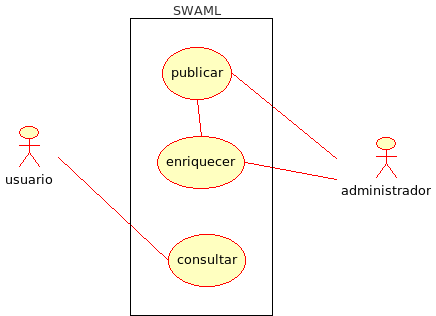
\includegraphics[width=12cm]{images/uml/casos-uso/general.png}
	\caption{Casos generales de uso}
	\label{fig:uml:casos-uso}
\end{figure}

Como se ve en la figura~\ref{fig:uml:casos-uso} se puede disntiguir claramente
tres grandes bloques de casos de uso:

\begin{itemize}
 \item Publicar los datos
 \item Enriquecerlos
 \item Consultarlos
\end{itemize}

\subsubsection{Casos de uso}\label{sec:casos-uso}

Refinando el diagrama anterior se identifican varios casos de uso que paso a
enumerar:

\begin{itemize}
 \item Parametrizar el sistema
 \item Publicar
 \item Enriquecer los datos
 \item Consular los archivos generados
 \item Consultar la información extra generada
\end{itemize}

Para pasar a describirlos más detalladamente:

\begin{itemize}

  \item \textbf{Parametrizar el sistema:}
 	\begin{itemize}
 	  \item \textbf{Descripción:} Este caso de uso representa la labor 
		que el usuario administrador debe realizar para configurar 
		correctamente el sistema.
 	  \item \textbf{Flujo de eventos:} El caso de uso comienza cuando el
		usuario administrador comienza a editar una configuración, 
		bien manualmente o mediante el asistente que acompaña al 
		software.
	  \item \textbf{Precondiciones:} Es necesario disponer de un mailbox
		a exportar.
	  \item \textbf{Postcondiciones:} Ninguna detectada.
	\end{itemize}

  \item \textbf{Publicar:}
 	\begin{itemize}
 	  \item \textbf{Descripción:} Representa la acción de publicación 
		propiamente dicha.
 	  \item \textbf{Flujo de eventos:} El proceso es un proceso por 
		lotes que a partir de una configuración genera una serie 
		de ficheros RDF. Internamente se divide en varios procesos:
		\begin{enumerate}
		 \item \emph{Parsear} el mailbox
		 \item Revisar la consistencia de todas las relaciones entre los distintos mensajes
		 \item Enriquecer la información
		 \item Exportar cada uno de estos mensajes en RDF
		 \item Exportar los suscriptores en RDF
		 \item Exportar los suscriptores en KML si fuese requerido
		 \item Exportar todos los indices
		\end{enumerate}
		FIXME: revisar, Diego dice que no se corresponden a un "flujo de eventos", 
		porque no hay interacción con el usuario.
	  \item \textbf{Precondiciones:} Disponer de una configuración correcta.
	  \item \textbf{Postcondiciones:} El directorio destino de la exportación
		debe poder \emph{consumirse} mediante otro servicio, como un 
		servidor \texttt{HTTP} (Apache o similar).
	\end{itemize}

  \item \textbf{Enriquecer los datos:}
 	\begin{itemize}
 	  \item \textbf{Descripción:} Representa la interacción del 
		sistema con otras bases del conocimiento externas, 
		principalmente los FOAF de los suscriptores a la lista 
		de correo, para enriquecer la información en determinados 
		aspectos.
 	  \item \textbf{Flujo de eventos:} Se tratar de un proceso que se 
		repite iterativamente con cada uno de los suscriptores:
		\begin{enumerate}
		 \item Buscar su FOAF
		 \item Si lo tiene:
		 \begin{enumerate}
		  \item	Enlazar al suscriptor con su FOAF
		  \item Consultar sus coordenadas geográficas
		  \item Consultar su foto
		 \end{enumerate}
		 \item Si no lo tiene continuar con el siguiente suscriptor
		\end{enumerate}
	  \item \textbf{Precondiciones:} Disponer de la lista de suscriptores 
		cargada en memoria.
	  \item \textbf{Postcondiciones:} Ninguna detectada.
	\end{itemize}

  \item \textbf{Consular los archivos generados:}
 	\begin{itemize}
 	  \item \textbf{Descripción:} Representa la interacción del 
		usuario con los datos generados. Desde una simple consulta 
		manual a los ficheros RDF generados, hasta realizar consultas 
		de una forma más sofisticada.
 	  \item \textbf{Flujo de eventos:} Con la información obtenida se 
		repetirá siempre el mismo flujo:
		\begin{enumerate}
		 \item consultar
		 \item leer
		 \item comprender
		 \item y/o desechar
		\end{enumerate}
	  \item \textbf{Precondiciones:} Disponer de la lista exportada a RDF.
	  \item \textbf{Postcondiciones:} Ninguna concreta.
	\end{itemize}

  \item \textbf{Consultar la información extra generada:}
 	\begin{itemize}
 	  \item \textbf{Descripción:} Este caso de uso representa la consulta 
		por parte del usuario de la información extra generada, por el 
		ejemplo los suscriptores en formato KML.
 	  \item \textbf{Flujo de eventos:}
		\begin{enumerate}
		 \item consultar
		 \item explotar
		\end{enumerate}
	  \item \textbf{Precondiciones:} Disponer de la información geográfica 
		de los suscriptores.
	  \item \textbf{Postcondiciones:} Explotación de estos datos, por ejemplo
		visualizandolos\footnote{\url{http://maps.google.es/maps?q=http://swaml.berlios.de/demo/subscribers.kml}}
		con Google Maps\footnote{\url{http://maps.google.es/}}.
	\end{itemize}

\end{itemize}



